\documentclass[answers]{exam}
\usepackage{texPreamble}
%\usepackage{showkeys}
\extraheadheight{0.0in}
\extrafootheight{0.0in}
% ----------------------------------------------------------------
\makeatletter
\title{Math1080\\ Unit 1 Formula reference sheet}
%\date{}

\pagestyle{headandfoot}
\firstpageheader{}{\@title}{}
\runningfooter{}{}{}

\makeatother
\begin{document}
  \begin{center}
    \textit{Note}: Let $f(x)$ and $g(y)$ represent the area between 2 functions where appropriate.
    %\renewcommand{\arraystretch}{1.35}
    \begin{tabular}{@{}l@{\hspace*{15pt} }*{2}{m{0.1\linewidth}m{0.30\linewidth}}@{}}
      \toprule[1.25pt]
      Velocity& \multicolumn{4}{l}{$F(b)-F(a)=\ds\int_a^b f(x)\,dx \hspace*{20pt}\Longrightarrow\hspace*{20pt} v(t)=v(0)+\int_0^t a(x)\,dx$}\\\midrule
      %
      \lnret[c]{Disk/Washer\\ $\pi r^2$}
      &$\begin{array}{l}
        x-\textnormal{axis}\\
        y=0
      \end{array}$&
      $\ds\int_a^b \pi\parens{R^2-r^2}\,dx$ & 
      $\begin{array}{l}
        y-\textnormal{axis}\\
        x=0
      \end{array}$&
      $\ds\int_c^d \pi\parens{R^2-r^2}\,dy$\\[15pt]
      &
      $\begin{array}{l}
        y=c
      \end{array}$&
      $\ds\int_a^b \pi\parens{(R-c)^2-(r-c)^2}\,dx$ & 
      $\begin{array}{l}
        x=c
      \end{array}$&
      $\ds\int_c^d \pi\parens{(R-c)^2-(r-c)^2}\,dy$\\\\[-0.8\baselineskip]
      & 
      \multicolumn{2}{c}{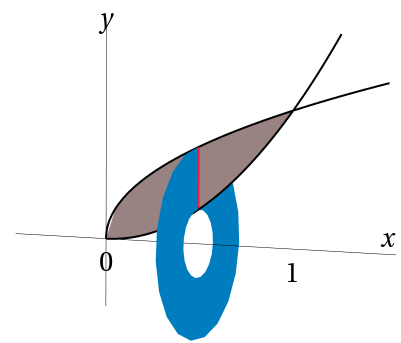
\includegraphics[width=0.175\linewidth]{washerMethod_x}}&
      \multicolumn{2}{c}{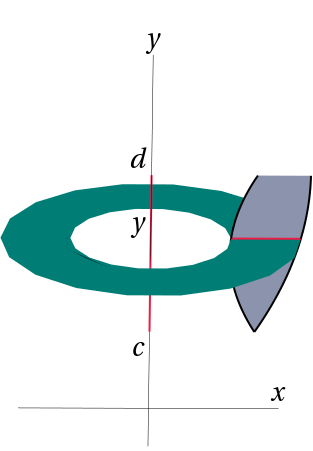
\includegraphics[width=0.175\linewidth,trim={0 0 0 110pt}, clip]{washerMethod_y}}\\\midrule
      %
      \multirow{4}{*}{\lnret[c]{Shell method\\$2\pi r\cdot h$}}& 
      $\begin{array}{l}
        x-\textnormal{axis}\\
        y=0
      \end{array}$&
      $\ds\int_c^d 2\pi y\cdot g(y)\,dy$ & 
      $\begin{array}{l}
        y-\textnormal{axis}\\
        x=0
      \end{array}$&
      $\ds\int_a^b 2\pi x\cdot f(x)\,dx$\\[15pt]
      &
      $\begin{array}{l}
        c<a\\
        y=c
      \end{array}$&
      $\ds\int_c^d 2\pi \parens{y-c}\cdot g(y)\,dy$ & 
      $\begin{array}{l}
        c<a\\
        x=c
      \end{array}$&
      $\ds\int_a^b 2\pi \parens{x-c}\cdot g(x)\,dx$\\[15pt]
      &
      $\begin{array}{l}
        b<c\\
        y=c
      \end{array}$&
      $\ds\int_c^d 2\pi \parens{c-y}\cdot g(y)\,dy$ & 
      $\begin{array}{l}
        b<c\\
        x=c
      \end{array}$ &
      $\ds\int_a^b 2\pi \parens{c-x}\cdot g(x)\,dx$\\\\[-0.8\baselineskip]
      &\multicolumn{2}{c}{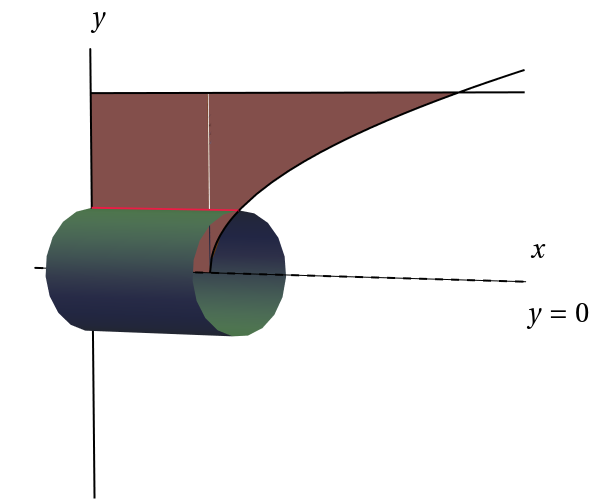
\includegraphics[width=0.175\linewidth,trim={0 0 0 50pt}, clip]{shellMethod_x}}&
      \multicolumn{2}{c}{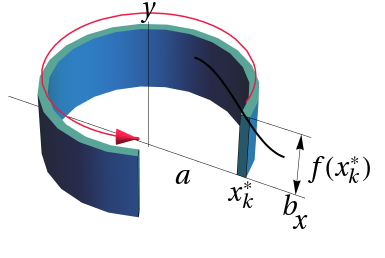
\includegraphics[width=0.175\linewidth]{shellMethod_y}}\\\midrule
      %
      \lnret[c]{Arc length\\$\sqrt{\parens{\frac{dx}{dx}}^2+\parens{\frac{dy}{dx}}^2}$}&& 
      $\ds \mathllap{L=}\int_a^b \sqrt{1+\sbrkt{f'(x)}^2}\,dx$\\\midrule
      %
      \lnret[c]{Surface area\\ $2\pi r\cdot h$}&&
      $\ds \mathllap{S=}\int_a^b 2\pi f(x)\sqrt{1+\sbrkt{f'(x)}^2}\,dx$\\\midrule
      \lnret[c]{Mass\\$\rho\cdot d$}&& $\mathllap{m=}\ds\int_a^b \rho\,dx$\\\midrule
      \lnret[c]{Work\\$F\cdot d$}&& $\mathllap{W=}\ds\int_a^b F(x)\,dx$\\\midrule
      Chain with load&& $\mathllap{W=}\ds\int_0^L \rho g (L-y)\,dy+ mgy$\\\midrule
      Pumping&& $\mathllap{W=}\ds\int_a^b \rho g A(y)(h-y)\,dy$\\\midrule
      Force-on-dam&& $\mathllap{F=}\ds\int _0^a\rho g\underbrace{(a-y)}_{\text{depth}}\underbrace{w(y)}_{\text{width}}dy$
      \\\bottomrule[1.25pt]
    \end{tabular}
  \end{center}
\end{document}
% ----------------------------------------------------------------
